
\documentclass[10pt,stdletter,dateno,sigleft]{newlfm}
\usepackage{pdfpages}
\usepackage{charter} % Use the Charter font for the document text

\newsavebox{\Luiuc}\sbox{\Luiuc}{\parbox[b]{1.75in}{\vspace{0.5in}
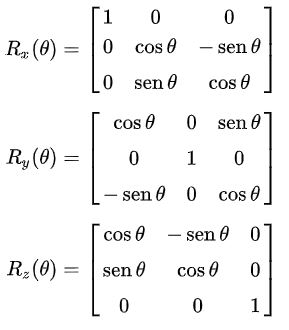
\includegraphics[width=1.2\linewidth]{MR.JPG}}} % LOGOTIPO DE LA EMPRESA EN LA PARTE SUPERIOR IZQUIERDA
\makeletterhead{Uiuc}{\Lheader{\usebox{\Luiuc}}}

\newlfmP{sigsize=50pt} % DISMINULLE EL CAMPO DE FIRMA

\lthUiuc % MUESTRA EL LOGO DE LA CNC logo

%----------------------------------------------------------------------------------------
%	YOUR NAME AND CONTACT INFORMATION
%----------------------------------------------------------------------------------------

\namefrom{Everardo Estrella} % Name

\addrfrom{
\date\\[27 de Septiembre del 2019] % Date
 \\ % Address
Matricez de Rotacion 
}

%----------------------------------------------------------------------------------------
%	ADDRESSEE AND GREETING/CLOSING
%----------------------------------------------------------------------------------------

\greetto{Simulacion de cinematica} 
\closeline{simulacion de cinematica directa e inversa de manipuladores seriales}

\nameto{ Everardo Estrella Rojo} 

\addrto{
Ingeneria en Mecatronica \\ 
Universidad Politecnica \\
Practica 3 \\
Cinematica de Robots
}

%----------------------------------------------------------------------------------------

\begin{document}
\date{FECHA 2019}
\begin{newlfm}

%----------------------------------------------------------------------------------------
%	LETTER CONTENT
%----------------------------------------------------------------------------------------
En la práctica de simulación de cinemática directa e inversa de manipuladores;  se dará a conocer La Matriz de Rotación para cada eje  cartesiano (x,y,z). A la bestia Ingresar a diferentes grados centígrados en cada rotación se practicará 10 traslaciones con la matriz de rotación simulado en matlab para obtener un resultado inequívoco.

\includepdf[pages=-]{21serial}


%----------------------------------------------------------------------------------------

\end{newlfm}

\end{document}